\section{Implementierung}

\begin{figure}[h]
 \centering
 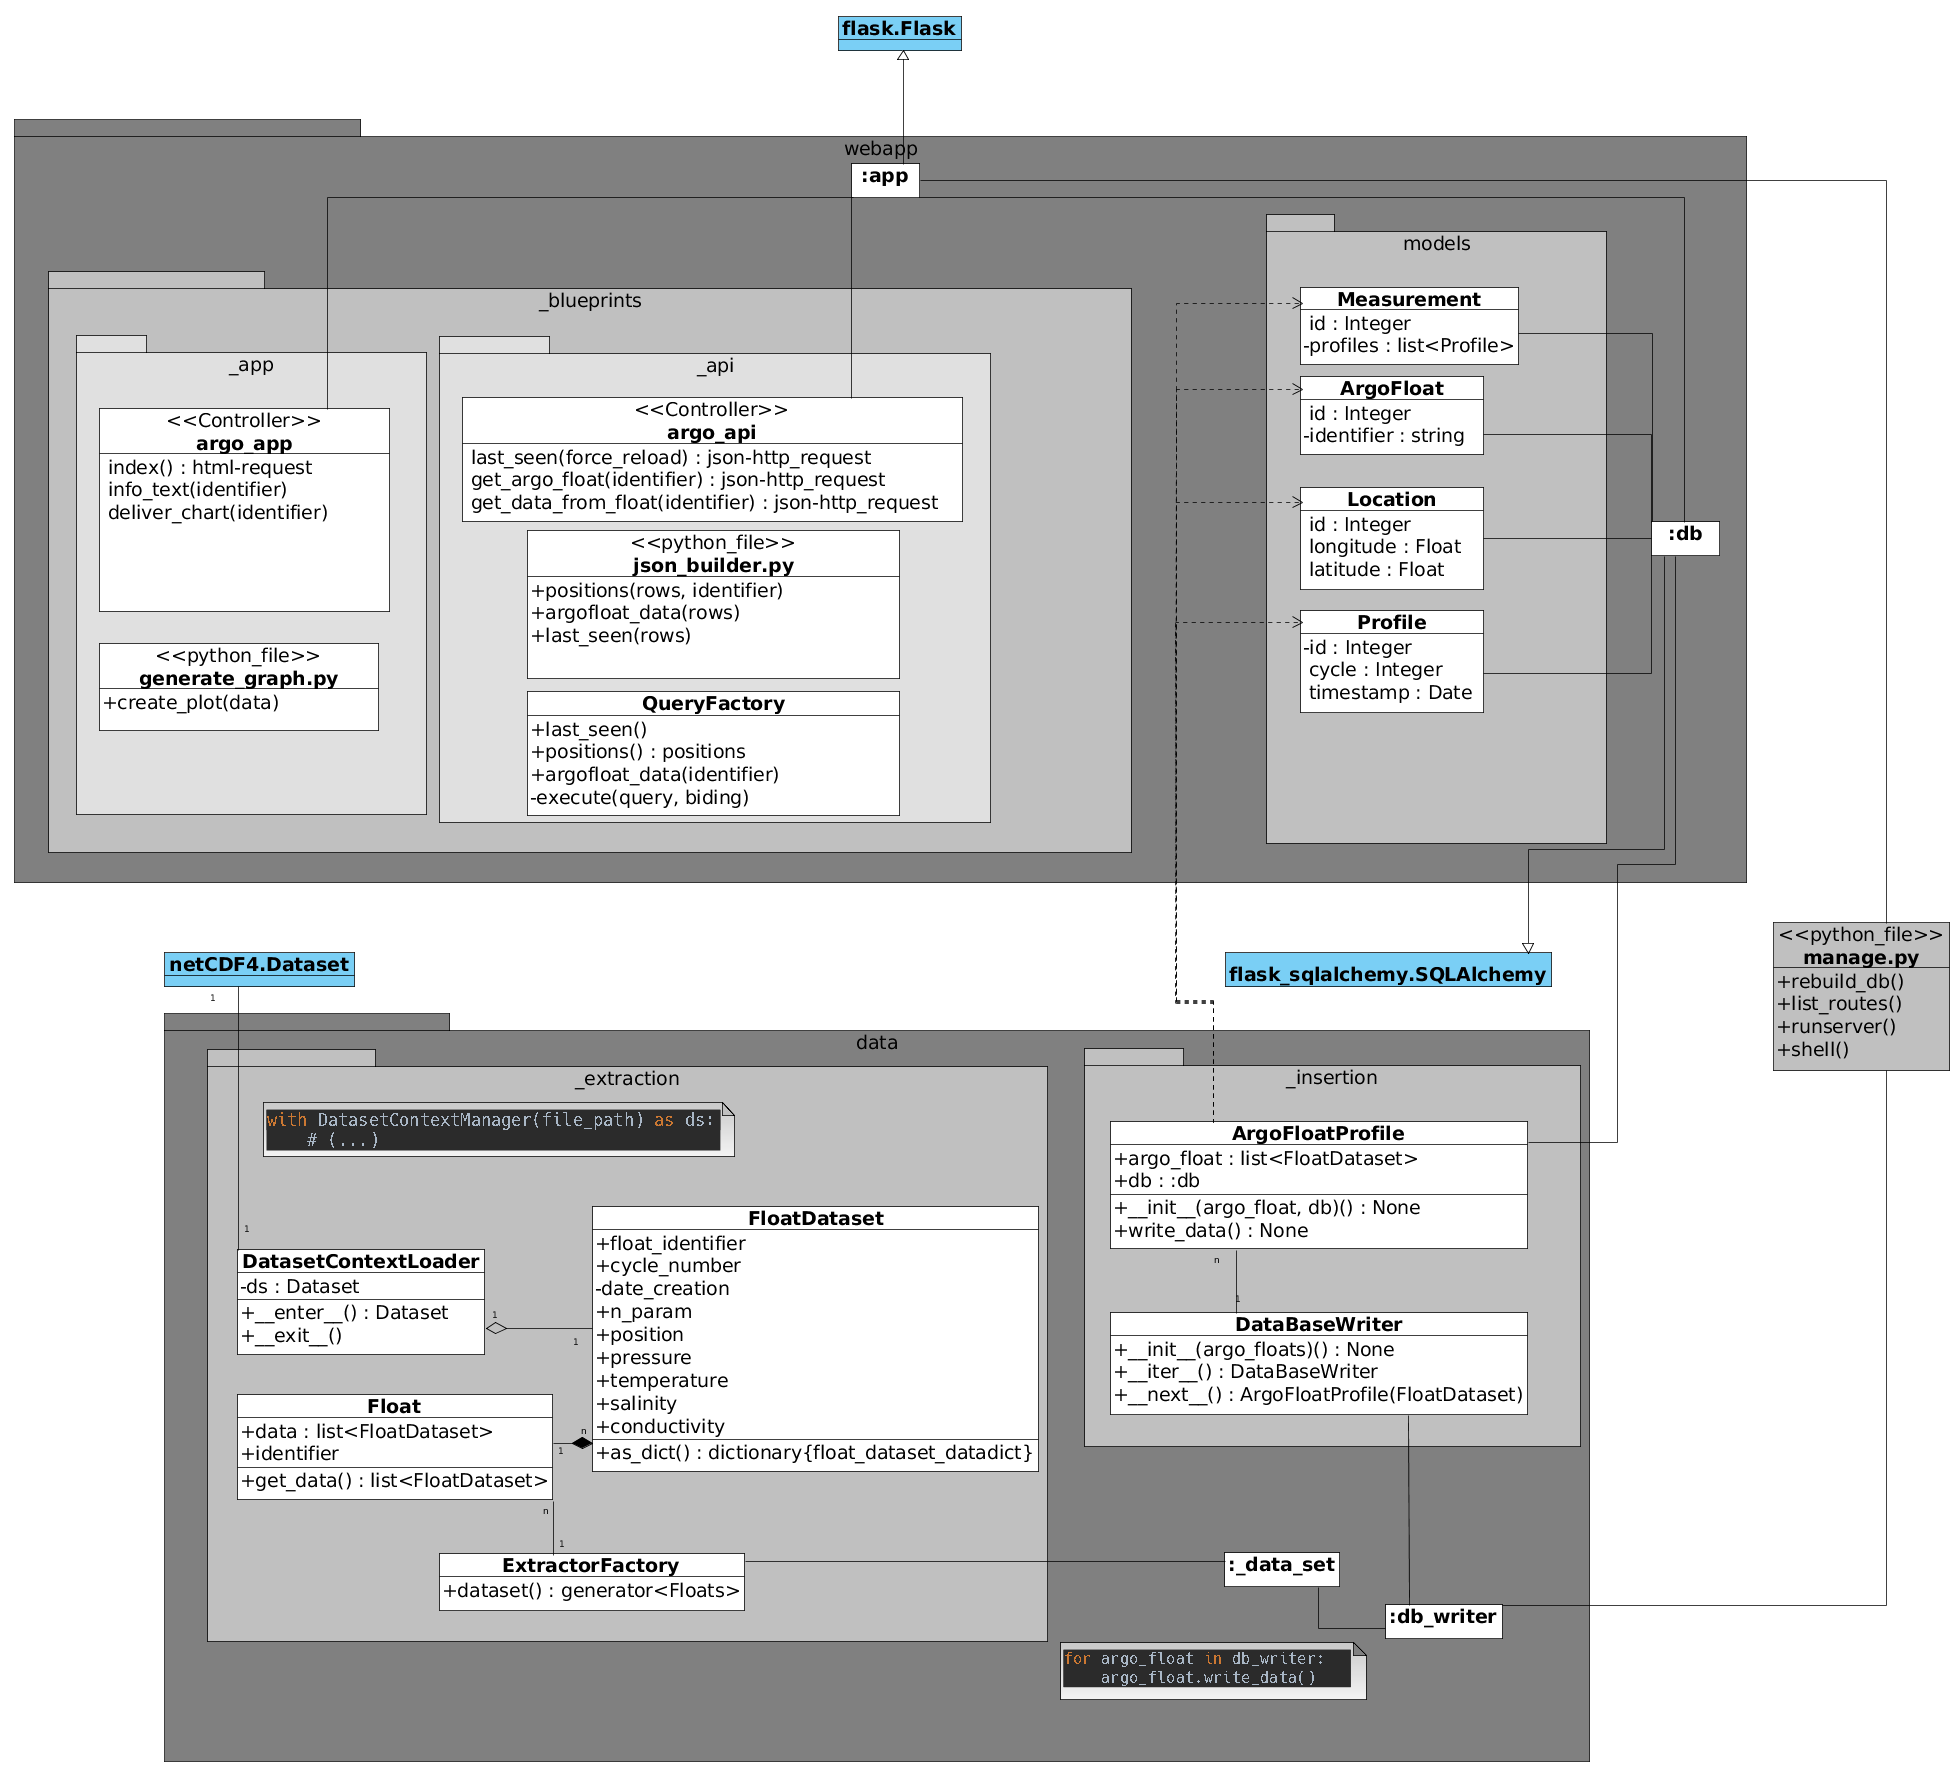
\includegraphics[width=\textwidth]{pix/Modulschema_komplett.png}
 % Modulschema_komplett.png: 876x911 px, 96dpi, 23.17x24.10 cm, bb=0 0 657 683
 \caption{Architekturbeschreibung von ArgoData}
 \label{fig:modulschema}
\end{figure}


% BEGIN DatenAGGREGATION
\subsection{Datenaggregation}


\subsubsection{Auslesen der Daten}

Der Datensatz besteht vor der Verarbeitung aus einer Ansammlung von Verzeichnissen und Dateien. Da die Gefahr besteht, dass geöffnete Dateien nicht wieder ordnungsgemäß geschlossen werden, muss eine Schnittstelle geschaffen werden, die unsachgemäße Verwendung der Dateien verhindert. Python sieht für diesen Zweck den Kontextmanager vor. In Listing \ref{lst:contextmanager} ist die hier verwendete Implementierung zu sehen.
\pagebreak
\pythonexternal[%
        caption={Kontextmanager zur Sicherstellung der richtigen Dateibehandlung.},
        label=lst:contextmanager]{./scr/beispiele/contextmanager.py}

In Listing \ref{lst:verwendungcontextmanager} ist die Verwendung des Kontextmanagers aufgezeigt und im Folgenden beschrieben.

\begin{python}[%
caption={Die Verwendung des Kontextmanagers},%
label={lst:verwendungcontextmanager}]
with DatasetContextManager(file_path) as ds:
    juld = ds.variables['JULD'][0]
\end{python}


Durch die Verwendung der Struktur über das Schlüsselwort \texttt{with} wird die Objektmethode \texttt{\_\_enter\_\_} aufgerufen. Diese gibt den objekteigenen \gls{netCDF}-Datensatz zurück. Dieses wird in der Verwendung im gleichnamigen Objekt \texttt{ds} gespeichert. Im darauf folgenden Operationsblock kann das Objekt nun verwendet und dessen Daten extrahiert werden. Nachdem der Operationsblock verlassen wurde, wird die Methode \texttt{\_\_exit\_\_} des Kontextmanagers aufgerufen. Innerhalb dieser Methode wird die Datei nun geschlossen.  Durch dieses Entwurfsmuster ist die richtige Verwendung der Datei also transparent sichergestellt. Ein Entwickler kann somit nicht durch Unachtsamkeit vergessen, den Datensatz zu schließen. Gleichzeitig erhöht sich die Lesbarkeit. Durch den Operationsblock ist jederzeit ersichtlich, ab welcher Stelle im Quelltext der Datensatz nicht mehr verfügbar ist.
Diese Schnittstelle wird in den Objektrepräsentationen der Argo-Floats und der Datensätzen verwendet, um auf die Daten zuzugreifen. In diesen wird die in Kapitel \ref{sec:entwurfAggregation} gezeigte Datenstruktur vorgehalten.


\subsubsection{Schreiben der Daten}

Um die Verarbeitung der Daten sowie den Prozess der Aggregation in der Datenbank richtig zu modellieren, ist es sinnvoll, den Prozess als Sequenz zu modellieren. Dies erlaubt es, die Datenstruktur über einen Generator vorzuhalten. Python sieht dafür den Iterator vor.
Die hier verwendete Implementierung ist in Listing \ref{lst:iteratorimpl} zu sehen. Das Interface wird über die Funktion \pythoninline{def __next__(self)} realisiert.
Dieses delegiert die Iteration zum Objekteigenen Generator \pythoninline{self.argo_floats}. In dem Moment, in dem ein Objekt aus dem Generator angefordert wird, findet die Verarbeitung der Datenstruktur statt.
Zum Schluss wird der Datensatz über ein Objekt ausgeliefert, das es erlaubt, die Daten in die Datenbank zu überführen.
Damit ist sichergestellt, dass der Prozess nur als Sequenz verwendet werden kann.

\pythonexternal[%
        caption={Implementierung des Iterators zur Steuerung der Aggregationssequenz}, label={lst:iteratorimpl}]{../BA_argo_proto/data/_insertion/_database_writer.py}

Die Verwendung der Schnittstelle ist in Listing \ref{lst:iterator_verwendung} aufgezeigt.

\pythonexternal[%
        caption={Verwendung der Schnittstelle zur Steuerung der Datenaggregation},
        label = {lst:iterator_verwendung}]{./scr/beispiele/lst-iterator-verwendung.py}



Eine zentrale Problemstellung im Prozess der Überführung der Daten in das relationale Schema ist die effektive Verwendung des flüchtigen Speichers. Eine klassische, sequenzielle Verarbeitung würde die Daten initial auslesen und diese in Gänze im Arbeitsspeicher vorhalten, bevor diese über den Mapper in die Datenbank überführt werden. Dieser Prozess wurde hier durch die Verwendung von Generatoren aufgebrochen. In Listing \ref{lst:dataextractor} ist die Implementierung dieser Schnittstelle zu sehen. Da in der Comprehension runde statt eckige Klammern verwendet werden, wird initial nur die logische Struktur als Sequenz vorgehalten. Die inhärenten Float-Objekte des Generators werden zu dem Zeitpunkt erzeugt, wenn diese durch eine Iteration aufgerufen werden. Damit werden die Daten erst zu dem Zeitpunkt ausgelesen, wenn diese für die weitere Verarbeitung benötigt werden.



Die Methode \texttt{get\_data\_sets()} erzeugt aus jedem Unterordner im definierten Arbeitsverzeichnis ein Float-Objekt und gibt dieses über das Schlüsselwort \texttt{yield} zurück. Durch diese Klasse wird somit ein Generator definiert, der es erlaubt, alle im Arbeitsverzeichnis definierten Argo-Float-Datenobjekte bereitzustellen, ohne diese bereits bei der Instantiierung kennen und abarbeiten zu müssen.


\pythonexternal[caption={Factory zur Extraktion der Datensätze},
                label={lst:dataextractor}]{/home/sebsch/Dokumente/Uni-Workdir/Bachelorarbeit/BA_argo_proto/data/_extraction/_data_extractor.py}




%END

\pagebreak
% BEGIN Webapp
\subsection{Webapplikation}

\subsubsection{Objektrelationales Mapping}\label{sec:implementierungORM}

% 1. Vorstellung SQL-Alchemy -- warum gewählt; Vor- und Nachteile

Als Objektrelationalen Mapper wird SQLAlchemy eingesetzt. Diese Software gilt als erprobt und wird bereits in einer Vielzahl von Softwaresystemen eingesetzt. So verwendet unter anderem reddit oder die Mozilla Foundation SQLAlchemy als Schnittstelle zur Datenhaltung. SQLAlchemy wird für die Verwendung in Flask empfohlen und es existiert eine Erweiterung, um die Verwendung des Mappers in Flask zu vereinfachen (vgl. \cite{openingtheflask} S. 33). \\
%% TODO Konzepte, Pattern und Nachteile von SQLAlchemy -- Pattern in Grundlagen zu ORM
%           1. LazyLoading
%           2. databinding
%           3. Foreign Key Mapping
%           4. rollback


% 2. Implementierung von Entitäten, und Relationen
In SQLAlchemy werden die Tabelleneinträge in Modellklassen abgebildet. In Listing \ref{lst:models_argofloat} ist die Implementierung des Models für eine ArgoFloat-Messstation zu sehen.

\pythonexternal[%                       -> SQLALCHEMY: ArgoFloat
    caption={Modellklasse für ein Argo-Float},%
    label={lst:models_argofloat}]%
    {/home/sebsch/Dokumente/Uni-Workdir/Bachelorarbeit/BA_argo_proto/webapp/models/_argo_float.py}

Die Registrierung des Models erfolgt über die Vererbung der Metaklasse \texttt{db.Model}. Die Eigenschaften der jeweiligen Entitäten werden über Attribute des Objektes implementiert. Diese werden in Instanzen von \texttt{db.Column} transferiert. Dies erlaubt das Festsetzen des Datentyps. So lassen sich auch weitere Datenspezifikionen definieren.  Die Attribute werden durch eine Parameterübergabe in den Initiator der Klasse mit Werten versehen.
Um das Binding umzusetzen, wurden Nachfahren der Modellklassen erzeugt. Diese benötigen für die Zuordnung das Attribut \texttt{\_\_bind\_key\_\_}.

Über das Schlüsselwort \texttt{db.relationship} werden Beziehungen beschrieben. In diesem Fall besteht eine $1 - N$ Beziehung  zu \texttt{measurements}($\mbox{argo\_float} \leftarrow \mbox{measurements}$)   (siehe auch Abbildung \ref{fig:ERM}). Als Übergabeparameter wird ein Name für die Beziehung erwartet. Der Parameter \texttt{backref} gibt den Namen der Klasse auf dem Mapper an. Diese Einstellung erlaubt den Aufruf der Beziehung auch in die entgegengesetzte Richtung. Der Parameter \texttt{lazy} definiert die verwendete Strategie für das Lazyloading. In diesem Fall wurde sich für \texttt{'dynamic'} entschieden. Diese Einstellung gibt bei Lesezugriffen ein vorkonfiguriertes Query-Objekt zurück. Dies erlaubt das Hinzufügen weiterer Filter vor dem Zugriff auf die Tabellen. Die durch diese Beziehung verbundene Modellklasse Measurements ist in Listing \ref{lst:models_measurement} zu sehen.

\pythonexternal[%                       -> SQLALCHEMY: measurement
    caption={Modellklasse für eine Messung},%
    label={lst:models_measurement}]%
    {/home/sebsch/Dokumente/Uni-Workdir/Bachelorarbeit/BA_argo_proto/webapp/models/_measurement.py}

Auf dieser Seite der Beziehung   $\left( \mbox{measurement} \to \mbox{argo\_float} \right)$ unterscheidet sich deren Implementierung. Für die eindeutige Zuordnung des übergeordneten Argo-Floats wird deren \texttt{id} als Fremdschlüssel registriert. Die Beziehung benötigt neben dem Namen der anderen Seite keine weiteren Parameter, da die Beziehung bereits konfiguriert worden ist.


% 3. Lesen und schreiben von Daten aus der Datenbank -- Rollbacks


Das Schreiben von Daten über den Mapper SQLAlchemy ist Teil der Datenaggregation. Der dort implementierte Programmcode ist in Listing \ref{lst:sqlalchemy_write} zu sehen.


\pythonexternal[%                       -> SQLALCHEMY: Schreiben
    caption={Das Schreiben der Daten eines Argo-Floats in die Datenbank},%
    label={lst:sqlalchemy_write}]%
    {/home/sebsch/Dokumente/Uni-Workdir/Bachelorarbeit/BA_argo_proto/data/_insertion/_argo_float_profile_writer.py}


Die hier implementierte Klasse \texttt{ArgoFloatProfile} ist für das Schreiben aller Datensätze eines ArgoFloats zuständig. Diese verwendet für die Zuordnung der Daten die Modell-Klassen aus der Webapplikation. Durch die Methode \texttt{write\_data} werden die Daten des durch \texttt{\_\_init\_\_} übergebenen Datensatzes in die Datenbank überführt.
Um ein dynamisches Binding realisieren zu können, wird der betreffende Parameter \texttt{bind} übergeben. Mithilfe dieses Parameters wird eine Session aufgebaut, welcher das Schreiben in die Datenbank erlaubt, die über das Binding definiert ist.

Für jeden Datensatz wird eine Instanz der betreffenden Modell-Klasse erstellt. Die dafür benötigten Daten werden aus den Datensätzen des Klasseneigenen Generator-Objektes \texttt{argo\_float} angefordert und als Parameter übergeben.

Der zuvor definierten Session werden nur die Instanzen der \texttt{Profile}-Klassen übergeben. Da alle zum Messprofil gehörenden Modells in diesem Kontext eindeutig sind, kann SQLAlchemy diese selbstständig zuordnen.
Zum Abschluss werden die Daten über \pythoninline{session.commit()} in die Datenbank überführt.
\pythoninline{session.rollback()} erlaubt es, die Veränderungen, die innerhalb dieser Session an der Datenbank herbeigeführt wurden, wieder auf den Urzustand zurückzuführen.  \\

SQLAlchemy bietet eine eigene Abfrage-Sprache an. In Listing \ref{lst:sqlalchemyreadquery} ist eine vereinfachte Implementierung der Abfage zur Bestimmung der Positionshistorie einer Argo-Float zu sehen, wie sie auch in der Web-API implementiert ist.

\pythonexternal[%                       -> SQLALCHEMY: Lesen 1
    caption={Anfragen über SQLAlchemy zum Lesen von Daten},%
    label={lst:sqlalchemyreadquery}]%
    {scr/beispiele/sqlalchemy_read.py}


In diesem Beispiel werden über eine Projektion auf Attribute von \texttt{ArgoFloat}, \texttt{Location} und \texttt{Profile} Daten angefordert. SQLAlchemy erlaubt die Definition von Joins über mehrere Tabellen. Diese werden durch die in den Modell-Klassen definierten Beziehungen aufgelöst. Die Selektion erfolgt durch die Methode \pythoninline{query.filter()}. In diesem Fall werden nur Relationen der Argo-Float mit dem identifier '1900037' ausgewählt. Die Methode \pythoninline{query.order\_by()} erlaubt das Sortieren der Ergebnisse. In diesem Fall werden die Datensätze durch das Attribut \texttt{Profile.timestamp} chronologisch sortiert.
\\

SQLAlchemy ist auch in der Lage, in SQL-Sprache definierte Anfragen zu verarbeiten. In Listing \ref{lst:sqlalchemyreadSQL} ist eine vereinfachte Implementierung aus der Web-API zu sehen. Diese extrahiert die letzten Positionen mit den dazugehörigen Zeitpunkten aus der Datenbank.

\pythonexternal[%                       -> SQLALCHEMY: Lesen 2
    caption={Das Ausführen von SQL Anfragen über SQLAlchemy},%
    label={lst:sqlalchemyreadSQL}]%
    {scr/beispiele/sqlalchemy_read_query.py}

Über die Methode \texttt{db.engine.execute()} können SQL-Queries direkt verarbeitet werden. Dies hat aber zwei entscheidende Nachteile. Der Query-Dialekt beschränkt die Anfrage auf ein bestimmtes \gls{DBMS}. Diese Anfrage ist für PostgreSQL entworfen und würde auf einem anderen \gls{DBMS} nicht funktionieren. Zum anderen würden Eingaben nicht gegen SQL-Injections gesichert werden. Eine Abfrage wie
\pythoninline{
db.engine.execute(f'SELECT * FROM argo\_floats WHERE argo_floats.identifier=\{user\_input\})
} würde also unabschätzbare Sicherheitsrisiken mit sich bringen.
\\

% 4. Einbindung von SQLALCHEMY in den Flask Kontext als Beispiel für zeitkritische import in flask



Flask bietet für die Einbindung von SQLAlchemy eine Erweiterung an.
Durch diese Erweiterung wird eine SQLAlchemy-Instanz durch ein zentrales und scheinbar globales Objekt (\texttt{db}) repräsentiert. Dies ermöglicht eine einfache Datenabstraktion und ist für Flask typisch. Dieser Mechanismus wird durch die zeitkritische und in ihrem Ablauf fest vorgeschriebene Erstellung von Objekten und Submodulen erkauft.
Dieser Prozess ist bei der Einbindung von \texttt{flask-sqlalchemy} gut sichtbar. Aus diesem Grund wird die Initialisierung dieser Erweiterung hier gesondert dargestellt.

In Abbildung \ref{fig:sequenzSQLALCHEMY} ist eine sequentielle Darstellung des Prozesses zu sehen und wird im Folgenden beschrieben.

\begin{figure}[H]
 \centering
 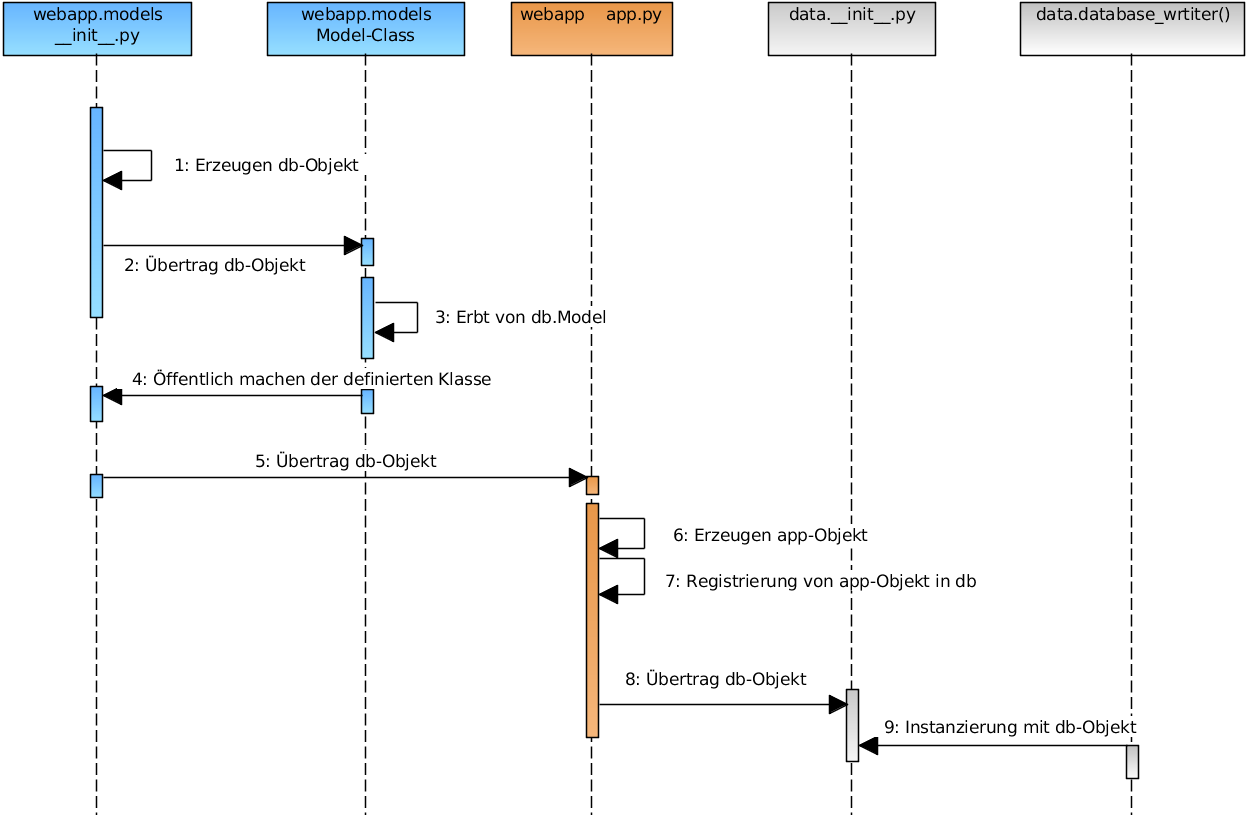
\includegraphics[width=\textwidth]{pix/seq_db.png}
 % seq_db.png: 1310x617 px, 96dpi, 34.66x16.32 cm, bb=0 0 982 463
 \label{fig:sequenzSQLALCHEMY}
 \caption{Sequenzdiagramm der Einbindung von SQLAlchemy}
\end{figure}


\begin{enumerate}
 \item
        In der Datei \texttt{webapp.models.\_\_init\_\_.py} muss sichergestellt werden, dass die SQLAlchemy-Instanz noch vor der Initiierung der Modell-Klassen erzeugt wurde.
 \item
        Nun kann das \texttt{db}-Objekt in die Modellklassen übertragen werden. Dafür importieren diese \texttt{db} in ihren Scope.
 \item
        Die Modell-Klassen werden in \texttt{db} registriert. Dafür erben diese von der Metaklasse \texttt{db.Model}. Siehe auch Listings \ref{lst:models_argofloat} und \ref{lst:models_measurement}.

        \pythonexternal[%
    caption={\texttt{webapp.models.\_\_init\_\_.py}},%
    label={lst:initpy_models}]{/home/sebsch/Dokumente/Uni-Workdir/Bachelorarbeit/BA_argo_proto/webapp/models/__init__.py}


 \item
        Die Modell-Klassen dürfen erst nach der Instantiierung von \texttt{db} über den Scope des Submodules heraus bekannt gemacht werden, um sicherzustellen, dass dieses bereits existiert. Die Implementierung des Ablaufs ist in Listing \ref{lst:initpy_models} ersichtlich.

 \item  \label{enum:seqdbwebapp1}
        Die Instanz \texttt{db} kann nun mit den in ihr registrierten Modell-Klassen  aus dem Submodul in die Datei \texttt{webapp.\_\_init\_\_.py} importiert werden.

\item
        Hier wird nun das globale Objekt der Flask-Instanz (\texttt{app}) erstellt und konfiguriert.

\item   \label {enum:seqdbwebapp3}
        Anschließend wird \texttt{app} in \texttt{db} registriert. Die Schritte \ref{enum:seqdbwebapp1} bis \ref{enum:seqdbwebapp3} können über das Listing \ref{lst:init_webapp} nachvollzogen werden.

\item   Die Instanz \texttt{db} aus dem Scope
        \texttt{webapp.db} ist nun fertig konfiguriert und kann für das Lesen und Schreiben in die Datenbank verwendet werden.
\end{enumerate}


\pagebreak
\subsubsection{Controller}

\pythonexternal[%
    caption={ \texttt{webapp.\_\_init\_\_.py}},%
    label={lst:init_webapp}]{/home/sebsch/Dokumente/Uni-Workdir/Bachelorarbeit/BA_argo_proto/webapp/__init__.py}

% 1. Vorstellung Flask -- warum gewählt; Vor- und Nachteile

Über die globale Instanz des \gls{Controller}s (\texttt{app}) kann auf Daten zugegriffen und die Konfiguration vorgenommen werden. In Listing \ref{lst:init_webapp} ist die Initialisierung des \gls{Controller}s zu sehen.
% 2. Trennung von \gls{API} und APP in verscheidene Blueprints

Über Blueprints wird die in Kapitel \ref{sec:entwurfRoutes} ausgearbeitete logische Trennung zwischen \texttt{app} und \texttt{api} realisiert. Die hier definierten Module umfassen auch die in diesem Kontext benötigten Hilfsprogramme. Die hier implementierte Modulstruktur von \texttt{argo\_api} und \texttt{argo\_app} ist im Folgenden ersichtlich.

\begin{description}
 \item [argo\_api] $ $

    \begin{description}
     \item [query\_factory]
        Alle lesenden Zugriffe zur Datenbank werden über eine QueryFactory zentral zusammengefasst. Die hier ausgearbeitete Implementierung ist in Kapitel \ref{sec:implementierungORM} ausführlich beschrieben.

     \item [json\_builder]
        Durch diese Programmabschnitte werden die Daten in Listen und Dictionaries überführt. Die Variablen und Datenstrukturen werden dabei so angelegt, dass diese direkt als JSON bzw geoJSON ausgeliefert werden können.
    \end{description}

    Dieses \gls{Controller}-Blueprint fordert die Daten über die \texttt{query\_factory} an und bringt sie über den \texttt{json\_builder} in das vorgesehene Format.  Die Umwandlung in JSON und die Erstellung des Requests erfolgt über \texttt{flask.jsonify}.
\pagebreak
 \item [argo\_app] $ $

    \begin{description}
     \item [generate\_graph] Dieser Programmteil erzeugt einen Plot über die Bibliothek \texttt{matplotlib}. Eine nähere Beschreibung der Erstellung findet sich in Kapitel \ref{sec:ImplementierungPLOTS}.
    \end{description}

    In diesem Blueprint werden Templates zu HTML-Dateien zusammengesetzt. Dafür benötigt dieser Programmteil Zugriff auf die Verzeichnisse für die jeweiligen Templates und statischen Dateien. Diese Daten werden über \texttt{flask.render\_template} zusammengesetzt und ausgeliefert.
\end{description}

Die so erstellten Blueprints werden im zentralen \gls{Controller} (\texttt{app}) über das Schlüsselwort \texttt{app.register\_blueprint} registriert und zusammengefasst.
Als zentrale Steuerungseinheit für den gesamten Programmablauf dient die Datei \texttt{manage.py}. Die Parameter dieser Datei werden im Folgenden kurz beschrieben:

\begin{description}

 \item [runserver] Durch diesen Parameter wird der Server der Applikation gestartet.


 \item [rebuild\_db] Dies stößt den Prozess der Datenaggregation an.  Streng genommen ist dies nicht Teil des \gls{Controller}s. Aus Gründen der Einfachheit wurde dieser Programmablauf aber in die Steuerungseinheit integriert.

 \item [shell] Durch diesen Parameter wird eine IPython-Shell gestartet. In diesem repl ist die Webapplikation mit all ihren Umgebungsvariablen initiiert. Diese Shell dient für das Debugging der Applikation.

 \item [list\_routes] Dieser Parameter listet alle Routen, die durch den Controller definiert sind auf der Kommandozeile auf.
\end{description}


\subsubsection{Templates}
% jinja2

Für das Erstellen der HTML-Dateien wurde die Template-Engine Jinja2 verwendet. Diese ist gut in Flask integriert. Jinja2 erlaubt das Modularisieren von HTML-Dateien, den Zugriff auf Variablen und übergebenen Daten sowie die Abarbeitung einfacher Strukturen und Wahrheitswerte.

% Modulare Struktur  ..?

Die Templatestruktur wurde in dieser Applikation stark modularisiert.  In Listing \ref{lst:templateMAP} ist der Einstieg in die Modulstruktur zu sehen und im Folgenden beschrieben.
\pythonexternal[%
    caption={ \texttt{webapp.templates.map.html}},%
    label={lst:templateMAP}]{/home/sebsch/Dokumente/Uni-Workdir/Bachelorarbeit/BA_argo_proto/webapp/templates/map.html}

Die Datei \texttt{\_base.html} ist für die Darstellung der Webseite verantwortlich. Diese wurde über Twitter Bootstrap realisiert. Als Vorlage diente dabei ein bereits ausgearbeitetes  \texttt{2-Column Layout} aus \cite{Ng2014}. Der Beispielcode wurde an die Anforderung der Applikation angepasst. Der Code wurde dabei in die logischen Bestandteile zerlegt und in die modulare Struktur der Webseite überführt. Der Code ist unter einer MIT Lizenz veröffentlicht. Damit kann der Code unter Nennung der Lizenz verwendet werden. Deswegen wurde ein Tag in das \gls{HTML} Element eingesetzt, um Autor und Lizenz zu nennen.

\subsubsection{Kartendarstellung}

 OpenLayers ist eine Programmbibliothek um interaktive Geoapplikationen zu entwickeln. Das \gls{Framework} ist in Javascript entwickelt und nimmt alle benötigten Berechnungen auf Clientseite vor. Die Bibliothek erlaubt es, Kartenmaterial aus verschiedensten Quellen zu rendern. Dabei können Kachel- oder auch Vektorbasierte Materialien eingebunden werden.
Die Elemente der Karte setzen sich, wie in Listing \ref{lst:olMap} zu sehen, zusammen.

\begin{javascript}[label={lst:olMap}, caption={Das ol.Map Element aus der Kartendarstellung}]
 var map = new ol.Map({
    layers: [mapVectorLayer, argoFloatsLayer],
    target: 'map',
    controls: ol.control.defaults({
        attributionOptions: false,
        zoom: false,
    }),
    view: new ol.View({
        center: [0, 0],
        zoom: 3.5,
        minZoom: 3
    })
});
\end{javascript}

Die Darstellung bassiert auf zwei Layern, einer Verktordarstellung der Kontinent- und Landesgrenzen (\texttt{mapVectorLayer}), sowie der Darstellung der ArgoFloats (\texttt{argoFloatsLayer}). Die Darstellung der Steuereinheiten wurde deaktiviert. Als Startposition wurden Längen- und Breitengrad mit jeweils 0 gewählt. Die Zoomstufe ist mit 3 initialisiert und es ist eine maximale Zoomstufe von 3.5 gewählt. Die Werte für die Zoomstufe wurden bei einer Auflösung von 1920x1080 ermittelt und getestet.
Die Karte bettet sich in das HTML-Element map ein und wird mit diesem zur Anzeige gebracht. Steuergesten mit Maus und Tastatur nimmt die Karte an dieser Stelle bereits entgegen.
\\
Der mapVectorLayer wurde aus der GeoJSON-Datei \texttt{countries.geo.json}  erstellt. Die Datei wurde von \cite{sundstrm16} heruntergeladen. Diese steht unter der Lizenz UNLICENSE und kann damit ohne Einschränkungen verwendet werden. Die Darstellung der Argo-Floats wird ebenso über eine GeoJSON realisiert. Diese wird auf dem Webserver über die \gls{api} bereitgestellt und wird über der URL \texttt{/last\_seen}  (siehe Listing \ref{lst:routesAPI}) angefordert. Die so angeforderte Datenstruktur hat ein spezifisches Format. In Listing \ref{lst:argGeoJson} ist das Format in einem gekürzten Format ersichtlich.

\begin{javascript}[label={lst:argGeoJson}, caption={Gekürzte geoJSON zur Darstellung der Argo-Floats}]
 {
"crs": {
    "properties": {
      "name": "EPSG:4326"
    },
    "type": "name"
  },
  "features": [
    {
      "geometry": {
        "coordinates": [
          -52.02875,
          12.92591
        ],
        "type": "Point"
      },
      "properties": {
        "feature_type": "latest_position",
        "identifier": "1901673",
        "last_seen": "Sun, 10 Feb 2013 00:00:00 GMT"
      },
      "type": "Feature"
    },
    // (feature_2, ..., feature_n)
    ]
}
\end{javascript}

Der Parameter \texttt{crs} (Coordinate Reference System Objects) bestimmt die Art der Kartenprojektion. Durch das property \texttt{EPSG:4326} wurde der GPS-Standard WGS84 - World Geodetic System 1984 eingesetzt. Dies deckt sich auch mit den durch die Messstationen bereitgestellten Geo-Koordinaten. Für die Darstellung werden diese Koordinaten in eine Merkatordarstellung (EPSG:3857) projiziert.
\\
Die Repräsentationen der Messstationen finden sich im Array \texttt{features}. Im Feld \texttt{geometry} werden Position und die Form des Features eingestellt. Über \texttt{properties} werden die zusätzlichen Daten \texttt{feature\_type}, \texttt{identifier} und \texttt{last\_seen} in diesem Format gespeichert.
Openlayers kann ein derartig formatiertes GeoJson selbstständig zur Anzeige bringen. Wie die Datei geladen wird, ist in Listing \ref{lst:argoFloatsLayer} zu sehen.
\pagebreak
\begin{javascript}[label={lst:argoFloatsLayer}, caption={Die Funktion argoFloatsLayer}]
var argoFloatsLayer = new ol.layer.Vector({
    style: FloatStyle,
    source: new ol.source.Vector({
        format: new ol.format.GeoJSON(),
        url: "/last_seen"
    })
});
\end{javascript}
Als Quelle für die Anzeigedaten wird hierbei ein \texttt{ol.source.Vector}-Objekt gewählt. Das Format und die \texttt{url} für die spezifizierte Datenquelle werden als Parameter übergeben.
Damit werden die ArgoFloats auf einer vektorbasierten Karte angezeigt.
\\
Was zu diesem Zeitpunkt noch fehlt, ist die Möglichkeit mit den ArgoFloats zu interagieren. Bei Hovern mit dem Mauszeiger über einer ArgoFloat soll ein Tooltip mit einigen Informationen erscheinen und die Messstation optisch hervorgehoben werden.  Die Hervorhebung wird durch den Befehl \jsinline{map.addInteraction(hoverInteraction)} in der Karte registriert. \texttt{overInteraction} ist eine Instanz von \jsinline{ol.interaction.Select} und erlaubt die Auswahl von Features und des Event-Typs. In diesem Fall werden alle Features des \texttt{argoFloatsLayer} ausgewählt, die unter dem Mauszeiger liegen. Openlayers wählt mit dieser Konfiguration einen Vergrößerungseffekt um das Feature hervorzuheben.

Um den Tooltip zur Anzeige zu bekommen, wurde eine weitere Funktion definiert. In Listing \ref{lst:pointermove} ist die Funktion für das Fangen eines \texttt{pointermove}-Events zu sehen.
\begin{javascript}[label={lst:pointermove}, caption={Das Abfangen eines pointermove-Events}]
map.on('pointermove', function (evt) {
    if (evt.dragging) {
        info.tooltip('hide');
        return;
    }
    displayFeatureInfo(map.getEventPixel(evt.originalEvent));
});
\end{javascript}

Die Funktion wartet auf definierte Eingaben. In diesem Fall wird der Funktionskörper durch das Bewegen des Mauszeigers über der Kartendarstellung ausgelöst. Der Event wird als \texttt{evt} in die innere Funktion überführt. Dort wird überprüft, ob es sich um einen dragging-event handelt. Ist dies der Fall, wird der DIV-Container mit der id \texttt{\#info} (\texttt{info}) ausgewählt und der darin liegende Tooltip über den CSS-Parameter \texttt{hide} versteckt. Diese Einstellung wurde gewählt, um störende Tooltips bei der Navigation mit der Karte zu unterbinden. In jeden anderen Fall wird der Pixel an der Spitze des Mauszeigers extrahiert und der Funktion \texttt{displayFeatureInfo} übergeben.
\\
\texttt{displayFeatureInfo} positioniert das info-Element in der Nähe des Mauszeigers und extrahiert etwaige unter dem Pixel liegende Features. Anschließend werden die Attribute des Features untersucht. Über den Befehl \jsinline{feature.get("feature_type") === 'latest_position'} werden Features aus dem \texttt{last\_seen}-GeoJson identifiziert. Ist die Identifikation positiv, werden weitere Attribute extrahiert und in den Text des Tooltips überführt. Zum Abschluss wird der Tooltip über seine CSS-Attribute zur Anzeige gebracht.

Die Funktion kann auch die Features der Positionshistorie einer Boje über einen Tooltip anzeigen. Da sich die hier darzustellenden Parameter unterscheiden, werden dessen Daten gesondert abgefragt.
\\

Die Interaktion über einen Klick passiert analog. In Listing \ref{lst:clickEvent} ist die hier verwendete Implementierung der Klick-Event-Abfrage gezeigt.
\begin{javascript}[label={lst:clickEvent}, caption={Das Abfangen eines Klick-Events}]
map.on('click', function (evt) {
    displayArgoData(map.getEventPixel(evt.originalEvent));
    displayPositions(map.getEventPixel(evt.originalEvent))
});
\end{javascript}

Auch an dieser Stelle wird die \texttt{map.on}-Funktion der Karte verwendet, um den Event abzufangen. Ist dieser vom Typ \jsinline{'click'}, so werden die darauf folgenden Funktionen mit dem Pixel an der Position des Mauszeigers aufgerufen. Im Folgenden wird der Programmablauf der hier aufgerufenen Funktionen erläutert:

\begin{description}
 \item [\texttt{displayArgoData}]
    Diese Funktion ist für die Darstellung der Messdaten, sowie des Informationstextes der ausgewählten ArgoFloat verantwortlich. Aus diesem Grund besteht sie aus zwei Unterfunktionen.
    \begin{description}
    \item [\texttt{display\_chart}]
        Diese Funktion stellt den Funktionsplot der Messwerte der ausgewählten ArgoFloat dar. Dafür wird am Anfang der div-Container mit der ID \texttt{\#chart-picture} ausgewählt. In diesem Container wird später das Bild platziert. Um bereits bestehende Bilder zu löschen, werden alle HTML-Elemente innerhalb des Containers erstellt. Anschließend wird das Bild der Messdaten über die Webroute /chart/[identifier]  (siehe Listing \ref{lst:routesAPI}) angefordert. Das Bild wird anschließend auf die Breite des Containers gebracht und der Bootstrap-Klasse \texttt{img-responsive} hinzugefügt. Damit wird das Bild formatiert über die Sidebar dargestellt.
    \pagebreak
    \item [\texttt{display\_info}]
        Diese Funktion stellt einen Info-Block zu den Metadaten der Argo-Float dar. Analog zum oberen Prozess werden hier Container aus dem DOM-Tree selektiert und das sich darin befindliche  \gls{HTML} manipuliert. Die Daten wurden hier als HTML-Objekte über einen Ajax-Befehl angefordert und direkt in den umliegenden Container injiziert.
    \end{description}

    Die oben genannten Funktionen werden aufgerufen, wenn es sich bei dem angeklickten Element um ein Feature vom Typ \texttt{Point} handelt. Der Bereich des Graphen wird an dieser Stelle sichtbar gemacht und der Info-Bereich eingeklappt. Die Sichtbarkeit der Sidebar wird ebenso an dieser Stelle eingestellt.

 \item [\texttt{displayPositions}]
    Diese Funktion stellt eine Positionshistorie einer spezifischen Messstation dar. Dafür wird ein GeoJSON über die url \texttt{/positions/[identifier]} angefordert. Das Sichtbar-Machen, der hier kodierten Daten geschieht analog zu der Darstellung aller Argo-Floats. Das GeoJson trägt zusätzlich noch ein \texttt{LineString}-Element, um den zeitlichen Verlauf der Positionen zu verdeutlichen.
\end{description}





\subsubsection{Zeichnen der Graphen} \label{sec:ImplementierungPLOTS}

% 1- verwendete Software, Vor und Nachteile, warum gewählt

Für die Darstellung der Messwerte wurde sich in dieser Applikation für die Python-Bibliothek \texttt{matplotlib} entschieden.  Diese Plotting-Engine ist in der Entwicklung von wissenschaftlichen Applikationen in Python sehr verbreitet.
Als Renderer wurde ein AGG-Renderer eingesetzt. Dieser erlaubt das Vorhalten der Bilddaten im Arbeitsspeicher, sowie deren Überführung in ein Canvas-Element.

In Listing \ref{lst:deliver_chart} ist die Funktion des \gls{Controller}s zu sehen, über die das Bild bereit gestellt wird.

\begin{python}[label={lst:deliver_chart}, caption={Ausliefern eines Funktionsplots Flask}]
@argo_app.route("/chart/<identifier>")
def deliver_chart(identifier):
    url = url_for('argo_api.get_argo_float', identifier=identifier, _external=True)
    data = requests.get(url).json()

    fig = create_plot(data)
    canvas = FigureCanvas(fig)
    png_output = BytesIO()
    canvas.print_png(png_output)
    response = make_response(png_output.getvalue())
    response.headers['Content-Type'] = 'image/png'

    return response
\end{python}
\pagebreak
Die Funktion wird im Blueprint \texttt{argo\_app} der Flask-Applikation mit der Route registriert. Als Parameter \texttt{identifier}  wird die eindeutige Identifikationsnummer der Messstation erwartet. Die zum Erstellen des Graphen benötigten Daten werden aus der \gls{api} angefordert. Dafür wird die URL der Datenschnittstelle der Methode \texttt{get\_argo\_float} in der \gls{api} ermittelt. Anschließend wird unter Zuhilfenahme der Python-Bibliothek \texttt{requests} der Datensatz über einen GET-Request angefordert. Die Methode \texttt{.json()} überführt die Daten von Json in eine Python-Datenstruktur.

\begin{description}
 \item [\texttt{create\_plot}]
    Diese Funktion ist für die Erstellung des Funktionsplots zuständig. Als Theme wurde sich hier für \texttt{'seaborn-whitegrid'} entschieden. Eine der damit vorgegebenen Grundeinstellungen wurden durch das Ändern der \texttt{rcParams} noch weiter angepasst.\\
    Für die Darstellung der drei Funktionsplots wurden jeweils ein Achsen-Objekt erstellt. Diese Achsen werden über ein Gridspec untereinander angeordnet.

    Die Datensätze werden über die Y-Achse aufgetragen, wärend die X-Achse die Zeitstempel aufzeigt. Enthält ein Datensatz Werte keiner numerischen Zuordnung (\texttt{\gls{nan}}), so wird davon ausgegangen, dass dieser Datensatz nicht vorhanden ist und diese Achse nicht gezeichnet. Überschreitet ein Datensatz den ihm zugeschriebenen Wertebereich, so wird der Wertebereich der Y-Achse fest eingestellt. Die hierfür benötigten Daten werden über die zentrale Flask-Instanz aus der Konfiguration angefordert.

    Um den Platz besser nutzen zu können, wird die Beschriftung der Y-Achse nur auf dem untersten Graphen aufgetragen. Dieser enthält die Werte für den Druck des umliegenden Wassers. Dieser Messwert sollte in jeder Boje enthalten sein, es ist also nicht davon auszugehen, dass dieser Wert nicht gezeichnet wird.

    Die Achsen werden über das Gridspec in einer \texttt{Figure} zusammengefasst und damit aus dem Funktionskontext zurückgegeben.
\end{description}

Der so erstellte Funktionsgraph wird als Canvas-Element in einen response eingebunden und über diesen ausgeliefert.






% 2- Anfodern der Daten aus der API
% 3- Ablauf -- halten der Figure im RAM AGG-Renderer
% 4- Aufbau der Plotfunktion
% 5- Bereistellung des Bildes über response

%END
